\section{Adaptation Architecture and Strategy}

The original Gabriel platform has been validated in meeting the
latency bounds of WCA applications in single-user
settings~\cite{chen2017empirical}.  Scalable Gabriel aims to meet these latency
bounds in multi-user settings, and to ensure performant multitenancy
even in the face of overload.  We take two complementary approaches to
scalability.  The first is for applications to reduce their offered
load to the wireless network and the cloudlet through adaptation.  The
second uses end-to-end scheduling of cloudlet resources to minimize
queueing and impacts of overload.  We embrace both approaches, and
combine them using the system architecture shown in
Figure~\ref{fig:arch}.  We assume benevolent and collaborative clients
in this paper, and leave the handling of malicious users to future work.

\subsection{System Architecture}

We consider scenarios in which multiple Tier-3 devices concurrently
offload their vision processing to a single cloudlet over a shared
wireless network.  The devices and cloudlet work together to adapt
workloads to ensure good performance across all of the applications
vying for the limited Tier-2 resources and wireless bandwidth.  This
is reflected in the system architecture shown in
Figure~\ref{fig:arch}.

Monitoring of resources is done at both Tier-3 and Tier-2.  Certain
resources, such as battery level, are device-specific and can only be
monitored at Tier-3.  Other shared resources can only be monitored at
Tier-2: these include processing cores, memory, and GPU.  Wireless
bandwidth and latency are measured independently at Tier-3 and Tier-2,
and aggregated to achieve better estimates of network conditions.

This information is combined with additional high-level predictive
knowledge and factored into scheduling and adaptation decisions.  The
predictive knowledge could arise at the cloudlet (e.g., arrival of a
new device, or imminent change in resource allocations), or at the
Tier-3 device (e.g., application-specific, short-term prediction of
resource demand).  All of this information is fed to a {\em policy
  module} running on the cloudlet.  This module (described in detail
in Section~\ref{sec: resource-allocation}) is guided by an external
policy specification and determines how cloudlet resources should be
allocated across competing Tier-3 applications.  Such policies can
factor in latency needs and fairness, or simple priorities (e.g., a
blind person navigation assistant may get priority over an AR game).

A {\em planner module} on the Tier-3 device uses current resource
utilization and predicted short-term processing demand to determine
which workload reduction techniques (described in
Section~\ref{sec:workload-reduction}) should be applied to achieve
best performance for the particular application given the resource
allocations.

\begin{table*}[]
    \small
    \begin{tabular}{|r|p{35ex}|p{43ex}|p{32ex}|}
    \hline&&&\\[0.1in]
    &{\normalsize\bf Question}  & {\normalsize\bf Example} & {\normalsize\bf Load-reduction Technique} \\
    & & & \\ 
    \hline
    1&How often are instructions given, compared to task duration? 
        & Instructions for each step in IKEA lamp assembly are 
            rare compared to the total task time, e.g., 6 instructions over 
            a 10 minute task.
        & Enable adaptive sampling based on active and passive phases. \\ \hline
    2&Is intermittent processing of input frames sufficient for giving instructions?
        & Recognizing a face in any one frame is sufficient for
whispering the person's name.
        & Select and process key frames.  \\ \hline
    3&Will a user wait for system responses before proceeding?  
        & A first-time user of a medical device will pause until  an instruction is received.
        & Select and process key frames. \\ \hline
    4&Does the user have a pre-defined workspace in the scene?
        & Lego pieces are assembled on the lego board. Information outside the board can
             be safely ignored.
        & Focus processing attention on the region of interest. \\ \hline
    5&Does the vision processing involve identifying and locating objects?
        & Identifying a toy lettuce for a toy sandwich.
        & Use tracking as cheap approximation for detection. \\ \hline
    6&Are the vision processing algorithms insensitive to image resolution?
        & Many image classification DNNs limit resolutions to  
            the size of their input layers.
        & Downscale sampled frames on device before transmission.    \\ \hline
    7&Can the vision processing algorithm trade off accuracy and computation? 
        & Image classification DNN MobileNet is computationally cheaper than ResNet, but less accurate. 
        & Change computation fidelity based on resource utilization. \\ \hline
    % 8&Is there inherent human-level latency for a state change?
    %     & It takes at least a few seconds for a human to drill a hole.
    %     & Frame sampling and processing suppression based on heuristics   \\ \hline
    8&Can IMUs be used to identify the start and end of user activities?
        & User's head movement is significantly larger when searching for a Lego block.
        & Enable IMU-based frame suppression. \\ \hline
    9&Is the Tier-3 device powerful enough to run parts of the processing pipeline?
        & A Jetson TX2 can run MobileNet-based image recognition in real-time.
        & Partition the vision pipeline between Tier-3 and Tier-2.   \\ \hline
    \end{tabular}
\vspace{0.1in}
    \caption{\small Application characteristics and corresponding applicable techniques to reduce load}
    \label{tab:questions-techniques}
\end{table*}

\subsection{Adaptation Goals}
 
For the applications of interest in this paper, the dominant class of offloaded
computations are computer vision operations, e.g., object detection with deep
neural networks (DNNs), or activity recognition on video segments. The
interactive nature of these applications precludes the use of deep pipelining
that is commonly used to improve the efficiency of streaming analytics.  Here,
end-to-end latency of an individual operation is more important than
throughput. Further, it is not just the mean or median of latency, but also the
tail of the distribution that matters.  There is also significant evidence that
user experience is negatively affected by unpredictable variability in response
times. Hence, a small mean with short tail is the desired ideal. Finally,
different applications have varying degrees of benefit or utility at different
levels of latency.  Thus, our adaptation strategy incorporates
application-specific utility as a function of latency as well as policies
maximizing the total utility of the system.


\subsection{Leveraging Application Characteristics}
\label{sec:workload-reduction}

WCA applications exhibit certain properties that distinguish them from
other video analytics applications studied in the past.  Adaptation
based on these attributes provides a unique opportunity to improve
scalability.

\textbf{Human-Centric Timing:} The frequency and speed with which
guidance must be provided in a WCA application often depends on the
speed at which the human performs a task step.  Generally, additional
guidance is not needed until the instructed action has been completed.
For example, in the RibLoc assistant (a medical training application),
drilling a hole in bone can take several minutes to complete.  During
the drilling, no further guidance is provided after the initial
instruction to drill.  Inherently, these applications contain {\em
  active phases,} during which an application needs to sample and
process video frames as fast as possible to provide timely guidance,
and {\em passive phases,} during which the human user is busy
performing the instructed step.  During a passive phase, the
application can be limited to sampling video frames at a low rate to
determine when the user has completed or nearly completed the step,
and may need guidance soon.  Although durations of human operations
need to be considered random variables, many have empirical lower
bounds.  Adapting sampling and processing rates to match these active
and passive phases can greatly reduce offered load.  Further, the
offered load across users is likely to be uncorrelated because they
are working on different tasks or different steps of the same task.
If inadvertent synchronization occurs, it can be broken by introducing
small randomized delays in the task guidance to different users.
These observations suggest that proper end-to-end scheduling can
enable effective use of cloudlet resources even with multiple
concurrent applications.

\textbf{Event-Centric Redundancy}: In many WCA applications, guidance
is given when a user event causes visible state change. For example,
placing a lamp base on a table triggers the IKEA Lamp application to
deliver the next assembly instruction.  Typically, the application
needs to process video at high frame rate to ensure that such state
change is detected promptly, leading to further guidance.  However,
all subsequent frames will continue to reflect this change, and are
essentially redundant, wasting wireless and computing resources.
Early detection of redundant frames through careful semantic
deduplication and frame selection at Tier-3 can reduce the use of
wireless bandwidth and cloudlet cycles on frames that show no
task-relevant change.

\textbf{Inherent Multi-Fidelity}: Many vision processing algorithms
can tradeoff fidelity and computation.  For example, frame resolution
can be lowered, or a less sophisticated DNN used for inference, in
order to reduce processing at the cost of lower accuracy.  In many
applications, a lower frame rate can be used, saving computation and
bandwidth at the expense of response latency.  Thus, when a cloudlet
is burdened with multiple concurrent applications, there is scope to
select operating parameters to keep computational load manageable.
Exactly how to do so may be application-dependent.  In some cases,
user experience benefits from a trade-off that preserves fast response
times even with occasional glitches in functionality.  For others,
e.g., safety-critical applications, it may not be possible to
sacrifice latency or accuracy.  This in turn, translates to lowered
scalability of the latter class of application, and hence the need for
a more powerful cloudlet and possibly different wireless technology to
service multiple users.

\subsection{Adaptation-Relevant Taxonomy}
\label{sec:taxonomy}

The characteristics described in the previous section largely hold for
a broad range of WCA applications.  However, the degree to which
particular aspects are appropriate to use for effective adaptation is
very application dependent, and requires a more detailed
characterization of each application.  To this end, our system
requests a manifest describing an application from the developers.
This manifest is a set of yes/no or short numerical responses to the
questions in Table~\ref{tab:questions-techniques}.  Using these, we
construct a taxonomy of WCA applications (shown in
Figure~\ref{figs:design-space}), based on clusters of applications along
dimensions induced from the checklist of questions.  In this case, we
consider two dimensions -- the fraction of time spent in "active"
phase, and the significance of the provided guidance (from merely
advisory, to critical instructions).  Our system varies the adaptation
techniques employed to the different clusters of applications.  We
note that as more applications and more adaptation techniques are
created, the list of questions can be extended, and the taxonomy can be
expanded.

\begin{figure}[]
    \centering
    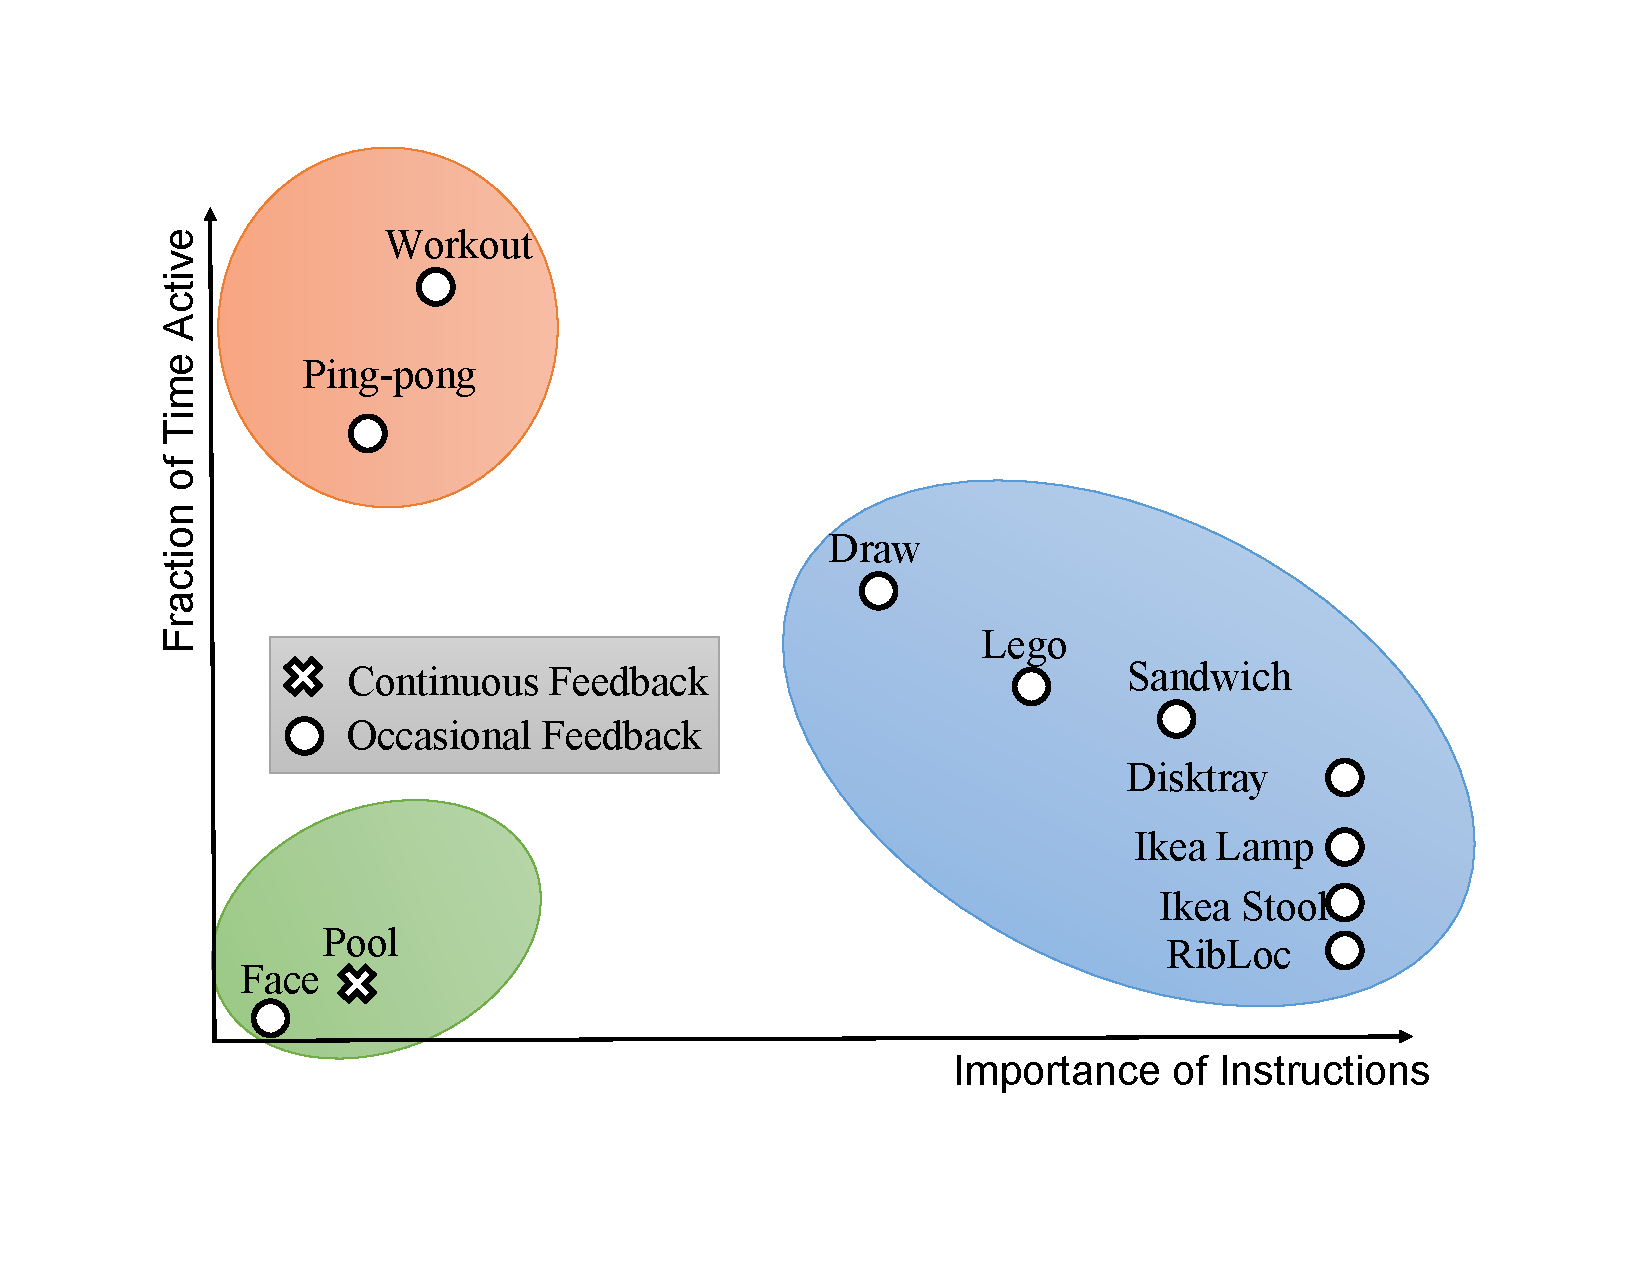
\includegraphics[width=1.1\linewidth, trim=14em 5em 6em 2em, clip]{FIGS/fig-design-space.pdf}
    \caption{\small Design Space of WCA Applications}
    \label{figs:design-space}
\end{figure}